\documentclass[12pt]{article}
\usepackage{graphicx}
% \usepackage[margin=1.0in]{geometry}

\usepackage{amsmath}
\usepackage{lipsum}
\usepackage{enumitem}
\setlist[itemize]{
  parsep=0pt,
  itemsep=0pt,
}

\usepackage[hang,flushmargin]{footmisc}

\usepackage{fancyhdr}
\pagestyle{fancy}
\lhead{Six Degrees of Wikipedia}

\title{Six Degrees of Wikipedia}
\author{Blake Appleby (aba2176)\\Jonathan Hall (jah2328)\\Ryan Wee (rw2800)}
\date{November 27 2023}

\begin{document}

\maketitle

\section*{1. Introduction}

The theory of ``six degrees of separation'' states that any two individuals are separated by at most six interpersonal connections. (In popular culture, one of these individuals is usually Kevin Bacon, and the other is some Hollywood actor.) In this project, we apply this theory to the dataset of Wikipedia pages. In particular, we say that Wikipedia page \textit{A} experiences \textit{one degree of separation} from Wikipedia page \textit{B} if and only if the contents of \textit{A} contain a hyperlink to \textit{B}. Given two arbitrary Wikipedia pages, our goal is thus to verify whether they are indeed connected by at most six degrees of separation. 

\section*{2. Overview}

It is quickly apparent that this is essentially a shortest path problem on a directed graph with fixed-weight edges. In particular, we can think of each Wikipedia page as a node, and each hyperlink on page \textit{A} to page \textit{B} as an edge from \textit{A} to \textit{B}. To solve this problem, we can do a naïve breadth-first search (BFS) from \textit{A}, and find the shortest path to \textit{B}.

\section*{3. Opportunities for Parallelization}

There is ample pre-existing material on how BFS can be parallelized.\footnote{See: en.wikipedia.org/wiki/Parallel\_breadth-first\_search, www3.nd.edu/$\sim$zxu2/acms\\60212-40212/Lec-07-2.pdf, and people.eecs.berkeley.edu/$\sim$demmel/cs267\_Spr16/Lectures/\\CS267\_March17\_Buluc\_2016\_4pp.pdf. Note that the tildes and underscores have to be manually replaced when copying these URLs into a browser, because LaTeX doesn't render tildes and underscores correctly.} The central idea is that breadth-first search can be represented using matrix algebra. In particular, represent the adjacency matrix as an $N$ by $N$ matrix $A^T$, where $A^T_{i,j}$ is $1$ if there is an edge from node $j$ to node $i$ and $0$ otherwise. Represent the current frontier as an $N$ by $1$ matrix $X$, where $X_{i,0}$ is $1$ if node $i$ is in the current frontier and $0$ otherwise. Then we can obtain the next frontier by taking $A^TX$. See the image below for more details.\footnote{Image taken from the Berkeley CS 267 PowerPoint.}

\begin{center}
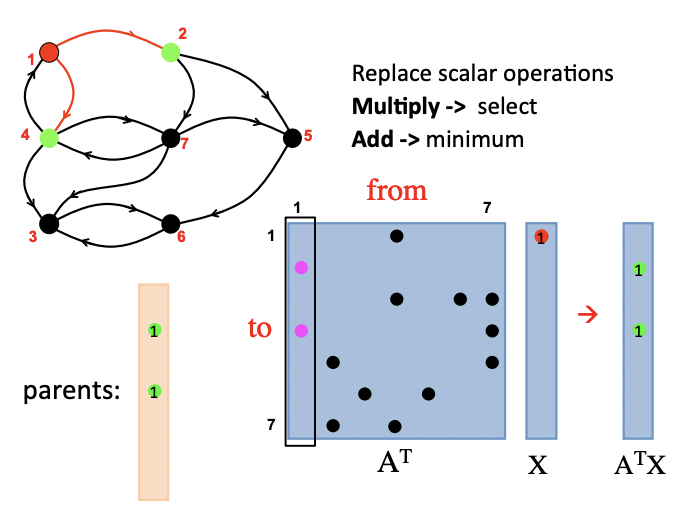
\includegraphics[width=0.5\textwidth]{matrix.png}
\end{center}

\noindent This matrix multiplication can be parallelized among $C$ cores by dividing the adjacency matrix $A^T$ into $C$ submatrices, either using 1-dimensional or 2-dimensional decomposition. 2-dimensional decomposition can be further optimized with direction optimization. Our plan is to implement as many of these strategies as possible, following the order above.

\section*{4. Opportunities for Scaling}

We can test our implementation on datasets of varying sizes by considering only a subset of all Wikipedia pages.

\end{document}
